\documentclass[11pt]{article}
\usepackage{bookmark}
\usepackage{algorithm}
\usepackage{algpseudocode}
\usepackage{amsfonts}
\usepackage{amsmath}
\usepackage{amssymb}
\usepackage{amsthm}
\usepackage{bm}
\usepackage{color}
\usepackage{comment}
\usepackage{float}
\usepackage{graphicx}
%\usepackage[hidelinks]{hyperref}
\usepackage{makecell}
\usepackage[caption=false,font=footnotesize,subrefformat=parens,labelformat=parens]{subfig}
\usepackage{wrapfig}
\usepackage{url}
\usepackage[table]{xcolor}
\graphicspath{{images_dd-mm2022/}}
\setlength{\parindent}{0.25in}
\setlength{\parskip}{.05in}
\pagestyle{plain}
%Title, date an author of the document
\title{Progress Report}
\author{Bardia Mojra}


\begin{document}
\maketitle
\thispagestyle{empty}

\bigskip
\bigskip
\begin{center}
 Robotic Vision Lab
\end{center}

\begin{center}
The University of Texas at Arlington
\end{center}

\newpage

\section{Specific Research Goals}
\begin{itemize}
      \item VPQEKF (\textcolor{red}{May 30th}): Work on the paper.
      \item DLO Manipulation Dataset (ICRA - \textcolor{red}{Sept. 1st})
\end{itemize}

\section{To Do}
\begin{itemize}
  \item QEKF Paper - 30\% extension (\textcolor{red}{June 30th}):
  \item Implementation (\textcolor{red}{May 30th}):
  \begin{itemize}
      \item Noise issue: noise cannot be modeled - revisit
      \item Rewrite RQuEst (RANSAC-QuEst) -- Done
      \item Replace the relative pose estimation routine in SfM example with RQuEst -- Done
      \item SfM: RQuEst cannot find solution -- under investigation
  \end{itemize}
  \item  DLO Manipulation:  \textcolor{red}{ICRA - Sept. 1st}
  \begin{itemize}
      \item Work on the paper everyday -- up-coming
      \item ICRA 2022 RL workshops: gym, stable-baseline3, and RL zoo -- on-going
      \item Setup digital twin reinforcement learing setup:
      \begin{itemize}
        \item Unity Robotics extension setup -- on-going.
        \item Design dynamic DLO data collection system.
        \item Build work cell. -- on-going
        \item Collect data and create a dataset.
        \item Define evaluation metrics.
        \item Create a high frequency RGBD dataset with UV-frames and open-loop input control actions as the ground truth.
      \end{itemize}
      \item Real-Time Preception
      \begin{itemize}
        \item Deep learning methods for keypoint pose estimation in real-time.
        \item Use UV dye dataset
        \item Use PVNet-like approach for known-object pose estimation.
      \end{itemize}
      \item Learning DLO Dynamics and System Identification
      \begin{itemize}
            \item List feasible approached for learing DLO dynamics
            \item Model dynamics and deformity in a latent space
      \end{itemize}
      \item Real-Time Control
      \begin{itemize}
        \item Time model inference, using auto-encoders generate the lowest
        dimensional representation for each object.
        \item Use another GAN model for object deformity for each object.
        \item Evaluate encoded representation for accuracy.
        \item Used another GAN to explore other abstraced representations from
        individual encoded representation. In theory, we can create a low
        dimensionsal representation for multiple similar objects, given all
        individual low-dimensional representations. This is inspired by "fundamental
        principles first" approach which has universal applicability.
      \end{itemize}
  \end{itemize}
\end{itemize}


\section{Progress}
The following items are listed in the order of priority:
\begin{itemize}
    \item XEst (\textcolor{red}{RAL ---}): I integrated Kaveh's QuEst algorithm
    into Matlab

    \begin{figure}[H]
      \begin{center}
        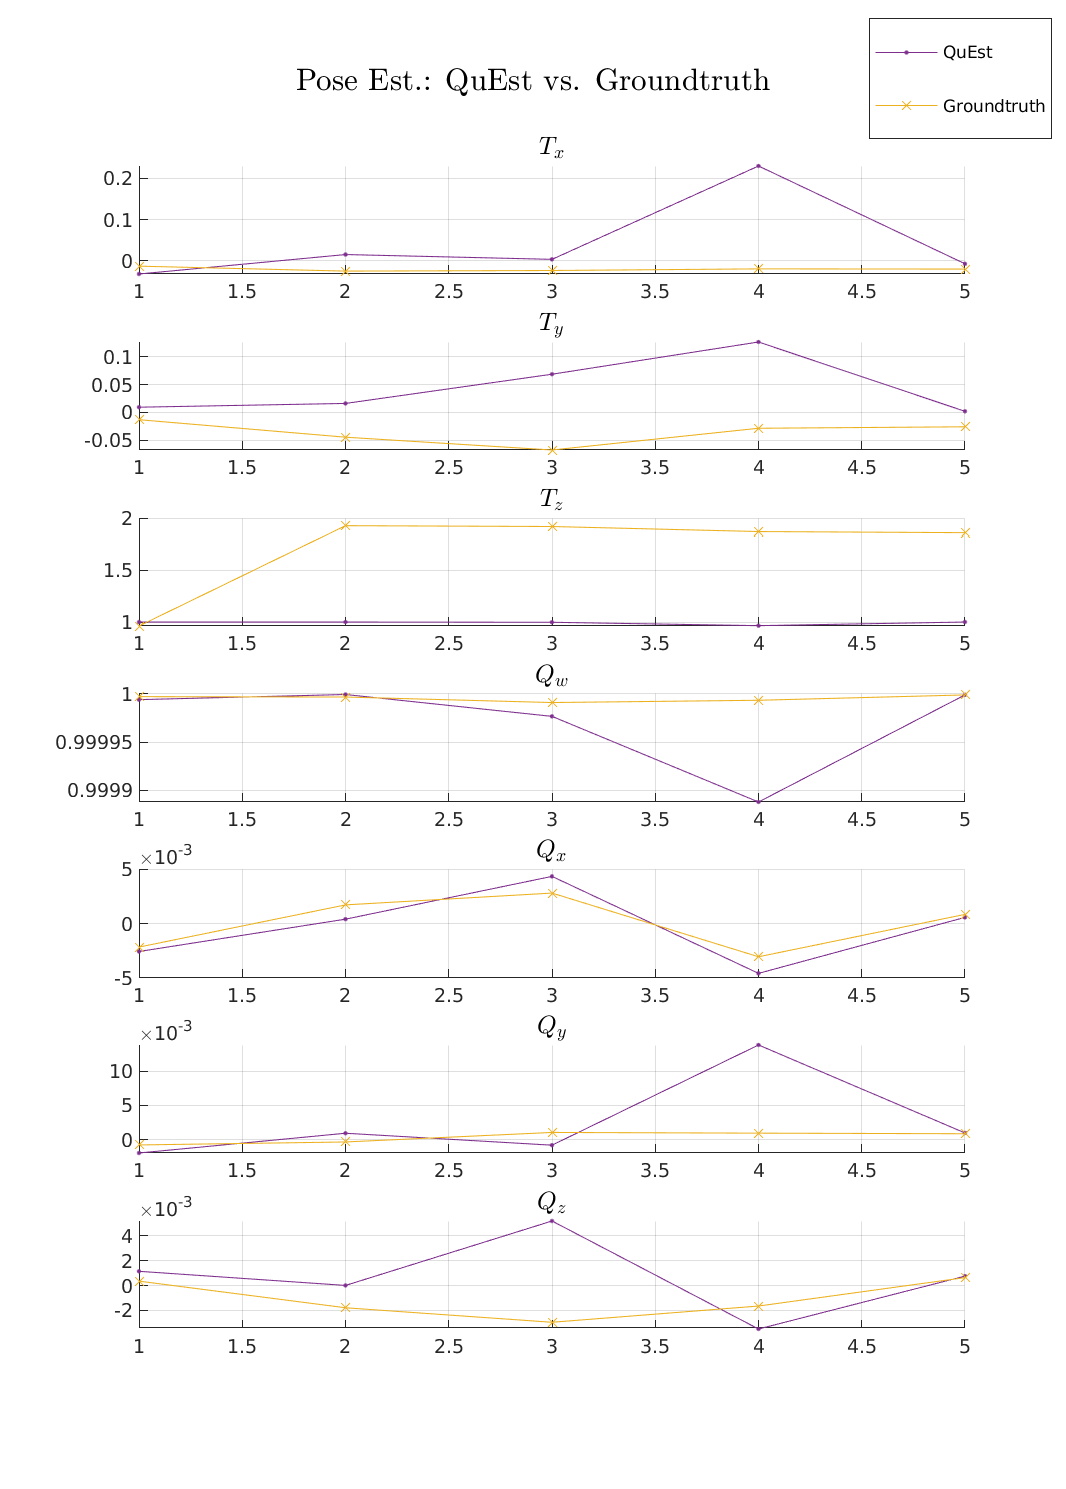
\includegraphics[width=\linewidth]{plt_pos_log_QuEst.png}
      \end{center}
      \caption{Pose module: Estimated pose log using QuEst.}
    \end{figure}

    \begin{figure}[H]
      \begin{center}
        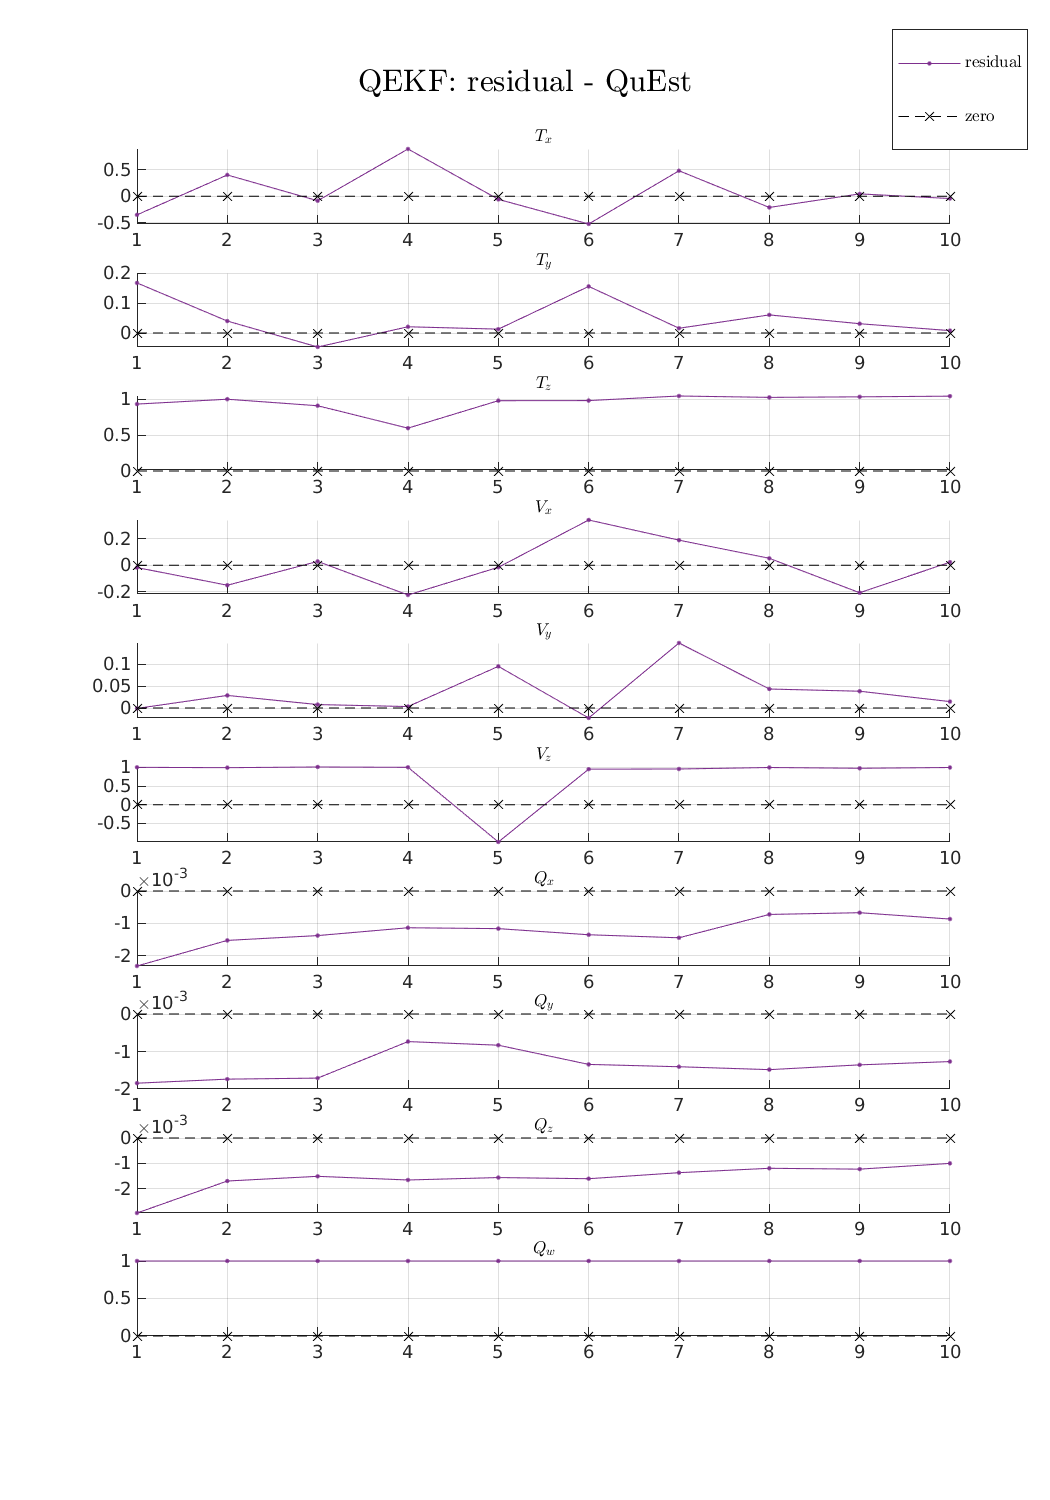
\includegraphics[width=\linewidth]{plt_qekf_log_residual_QuEst.png}
      \end{center}
      \caption{QEKF module: State ($T_{xyz},~V_{xyz},~Q_{xyzw}$) residual log
      with QuEst estimations as state measurements.}
    \end{figure}

    \begin{figure}[H]
      \begin{center}
        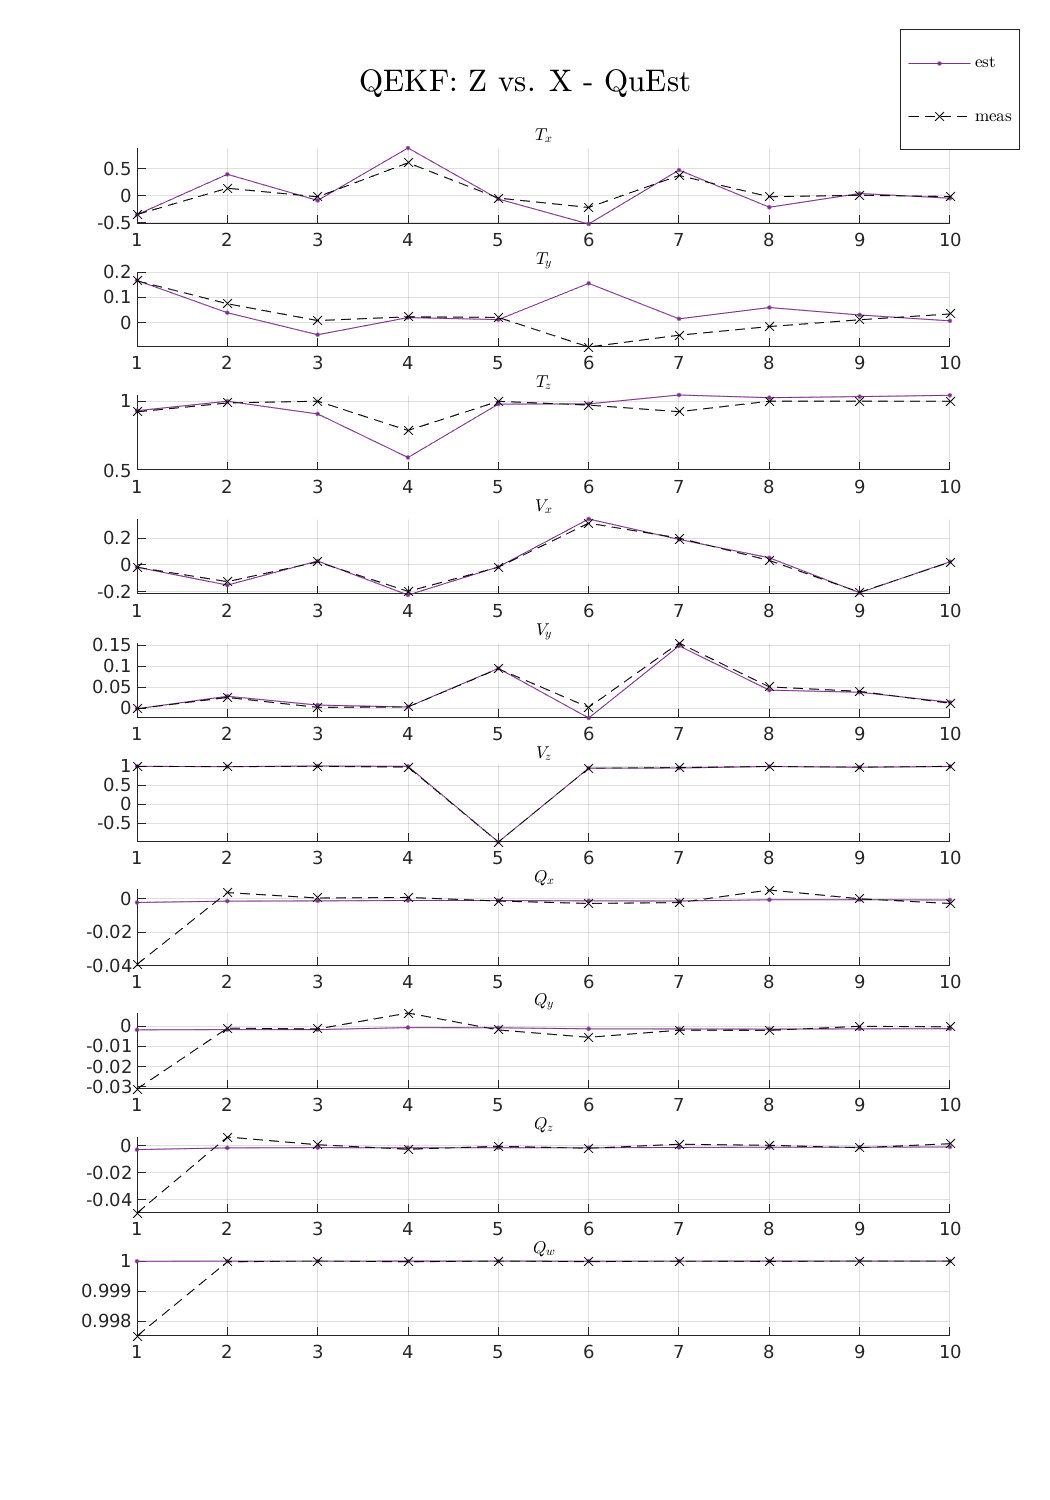
\includegraphics[width=\linewidth]{plt_qekf_log_ZvsX_QuEst.png}
      \end{center}
      \caption{QEKF module: State measurement vs. state estimation for QuEst.}
    \end{figure}

    Regarding our direction moving forward, I believe Dr. Gans and I have a
    made new realization. EKF remains one of the state-of-the-art
    methods for real-time state estimation with at least partially known
    dynamic model and completely known navigation environment. But related
    implementations for VSLAM and Structure from Motion (SfM) rely on \emph{Pose Graph},
    \emph{loop closure} via \emph{place recognition}, and two \emph{Bundle Adjustments}
    (one local and during run-time, the other at post processing).
    Related work by Nister \cite{nister2004efficient} makes no mention of
    EKF, loop closure, nor pose graph but based on my understanding I believe
    they implemented a variation of VSLAM or SfM. I was able to successfully run
    VSLAM and SfM in Matlab. Figures 4-5, 6-8
    show the outputs for VSLAM and SfM, respectively. Right now, I am in the
    process of rewriting the relative pose estimation algorithm to use QuEst
    with RANSAC (RQuEst) and triangulation instead of Sampson distance.
    Triangulation is a more robust method for finding the correct solution as
    Sampson distance is affected by noise. Moreover, they use pose graph and
    have a much more advanced method for point feature matching,
    keyframe selection, and view tracking which I am adopting.


    \begin{figure}[H]
      \begin{center}
        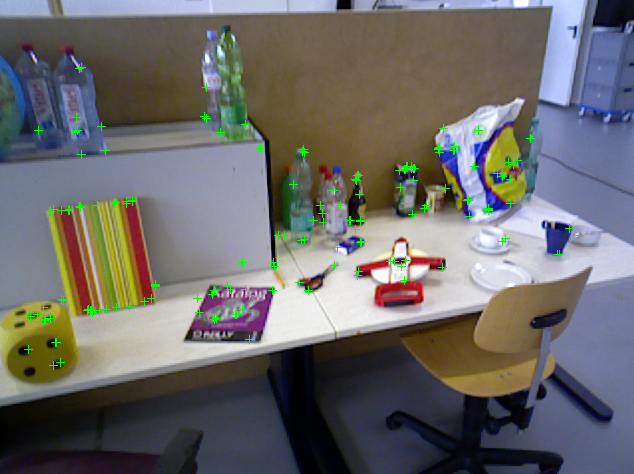
\includegraphics[width=.6\linewidth]{VSLAM_pFeats.png}
      \end{center}
      \caption{VSLAM: Final frame matched point features.}
    \end{figure}

    \begin{figure}[H]
      \begin{center}
        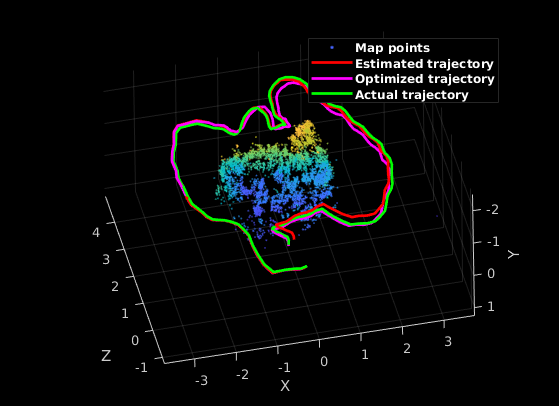
\includegraphics[width=.6\linewidth]{VSLAM_track.png}
      \end{center}
      \caption{VSLAM: Final track.}
    \end{figure}


    \begin{figure}[H]
      \begin{center}
        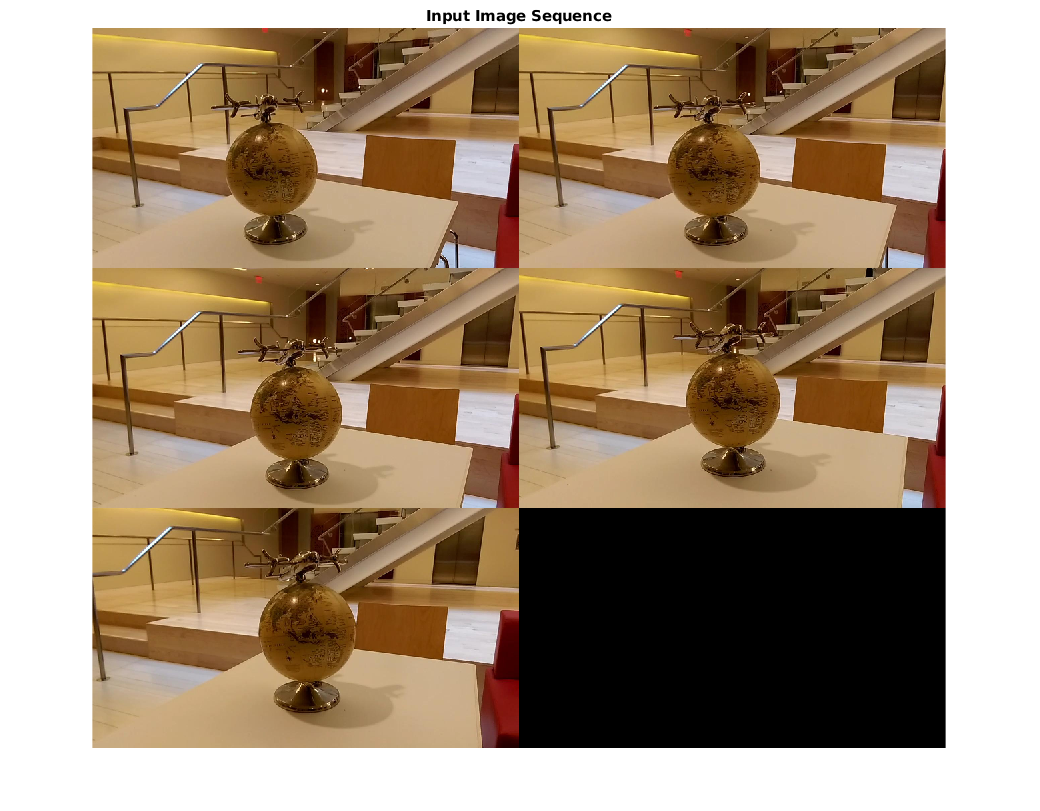
\includegraphics[width=.6\linewidth]{input_img_sequence.png}
      \end{center}
      \caption{SfM: Input image sequence.}
    \end{figure}

    \begin{figure}[H]
      \begin{center}
        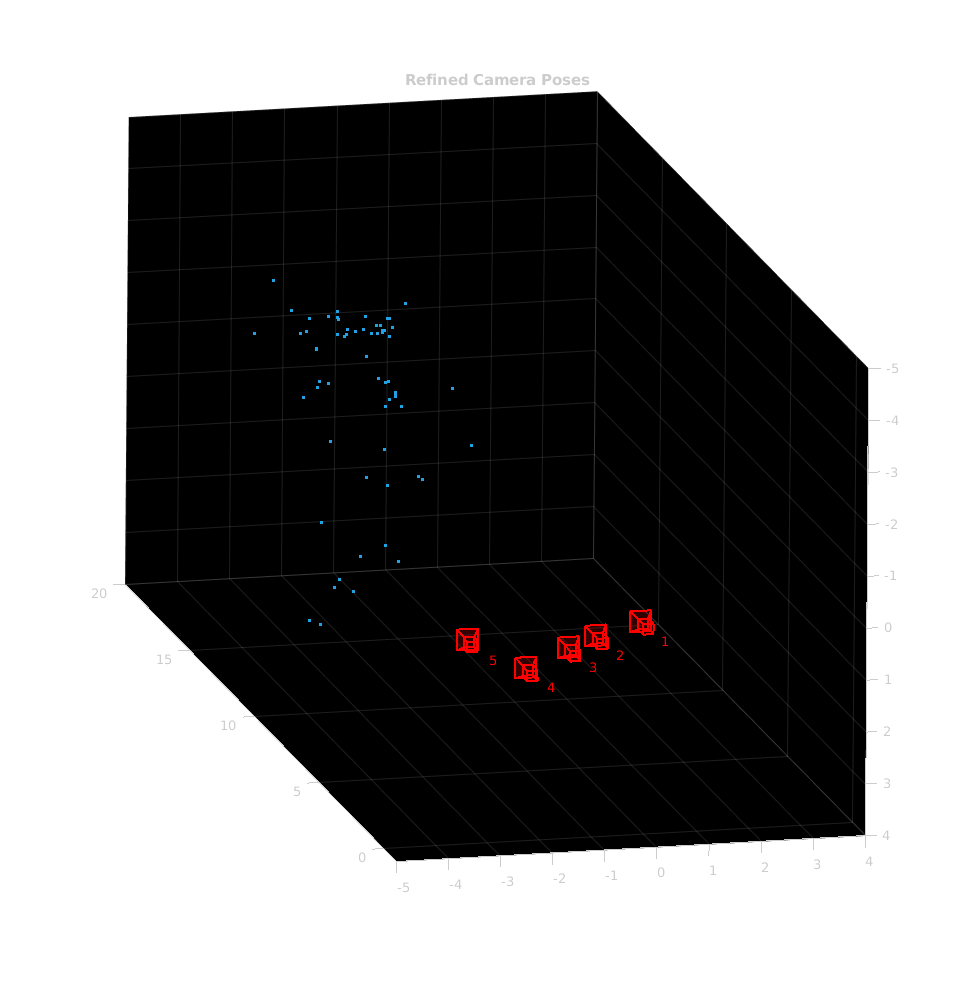
\includegraphics[width=.6\linewidth]{refined_cam_poses.png}
      \end{center}
      \caption{SfM: Refined camera poses.}
    \end{figure}

    \begin{figure}[H]
      \begin{center}
        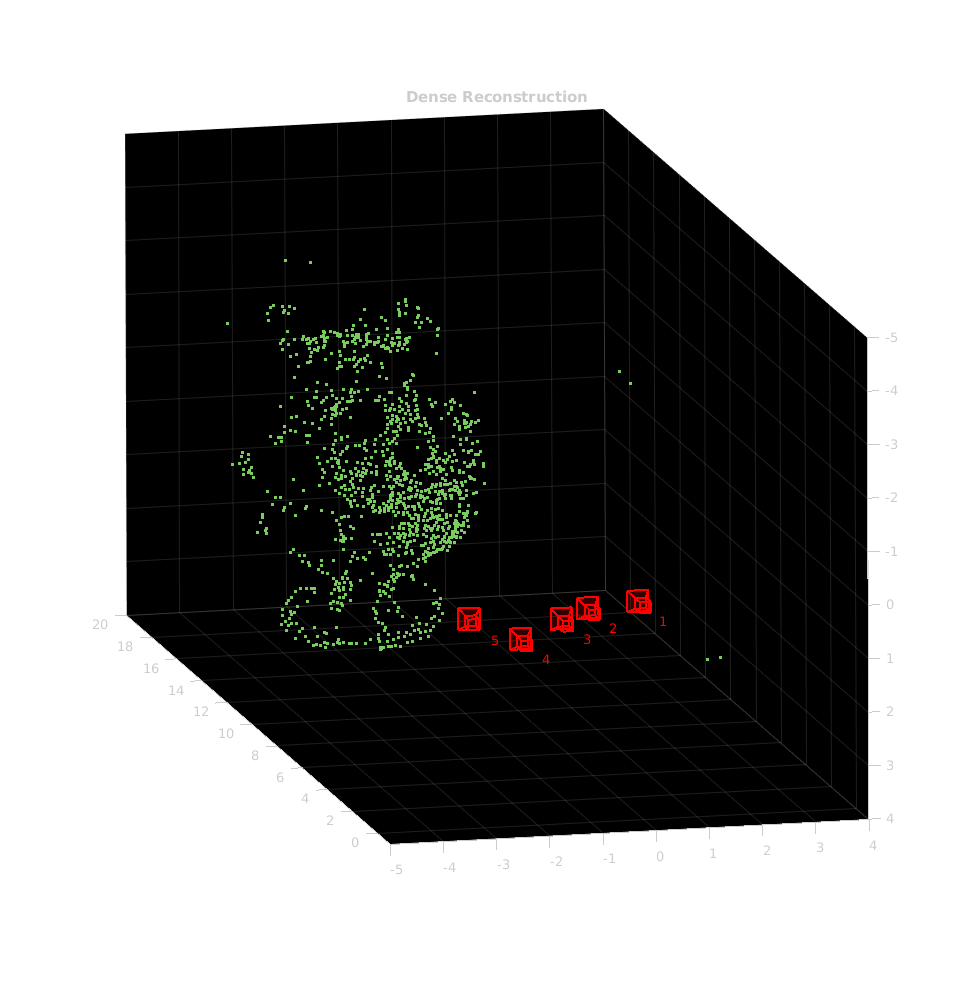
\includegraphics[width=.6\linewidth]{dense_reconstruct.png}
      \end{center}
      \caption{SfM: Dense reconstruction.}
    \end{figure}



    \item XEst - Semantic segmentation (\textcolor{red}{RAL - April 30st, 2022}):
    No update on implementing \cite{ballester2021dot}.
    \item DLO Dataset: I finished tutorials on Unity and learned basic C\# syntax.
    I also looked into Omniverse and Isaac Sim and decided to switch to that.
    I will have to install on TACC and asked Linus and Maicol to create their
    own accounts as well. I learned about a major shortcut that eliminates much
    of the need for setting up ROS. In one of the views, the presenting Nvidia
    engineer use Jupyter Noteboot to directly interface with a real robotic
    arm and synced its digital twin with physical arm which he controlling via
    real-time input. More

    \item Linus (REU): He will start on ROS2 tutorials soon.
    \item Maicol (REU): He will start on TurtleBot tutorials soon.
    \item Myself (with REU): I will set up Omniverse on TACC and VNC connection this week.

    \item DLO Control (MuJuCo): No update.

    \item Grasping Project (\textcolor{blue}{DLO-03}): I am making this a part of the DLO project.
    \item PyTorch Tutorials: Transfer learning.
    \item Manifold learning: Marcus emailed me some papers, I will read them
    and reply to him. I am not particularly interested in the project but his
    ideas are interesting and I would like to help him if I can. He is very
    knowledgeable on mathematics and I cherish that.

  \end{itemize}

\section{Intermediate Goals - Fall 2021:}
\begin{itemize}
      \item QEKF: Finish paper.
      \item UR5e: Do the tutorials.
\end{itemize}

\newpage

%Sets the bibliography style to UNSRT and import the
\newpage
\bibliography{ref}
\bibliographystyle{ieeetr}

\end{document}
